\documentclass[sigconf]{acmart}
% Local stand-in for the template's preamble.tex (same commands, used to compile outside Overleaf).
\usepackage{graphicx}
\usepackage{booktabs}
\usepackage{xcolor}
\newif\ifguideStyle
\newcommand{\guide}[1]{\ifguideStyle{\color{gray!65}\itshape #1}\fi}
\setcopyright{none}
\settopmatter{printacmref=false}
\renewcommand\footnotetextcopyrightpermission[1]{}
\pagestyle{plain}
\acmConference{}{}{}
\acmDOI{}
\acmISBN{}


% Guide styling: \guideStyletrue = show gray italic hints; \guideStylefalse = omit them
% \guideStyletrue
\guideStylefalse

\begin{document}

\title{Propose, Refine, Select: Annotator-Aware Instance Segmentation of Solar Filaments}
\subtitle{A Solution to the Solar Filament Segmentation Challenge 2026} % DO NOT CHANGE

\author{Omkar Kabde}
\affiliation{%
  \country{India}
}
\email{omkarkabde@gmail.com}

\begin{abstract}
This report describes our solution to the Solar Filament Segmentation Challenge~2026, a Kaggle competition on automatic segmentation of solar filaments in GONG H-$\alpha$ observations. Annotators of the MAGFiLO dataset agree only moderately on which structures are filaments (one annotator scored against another reaches a Panoptic Quality of 0.34), so we split the task into recall-oriented proposal, per-instance mask refinement, and a learned decision that keeps an instance when its expected matched IoU over annotators is high enough to raise Panoptic Quality. Two YOLO11s-seg detectors propose boxes, box-seeded U-Nets segment each box, a gradient-boosted model selects instances, and a second U-Net re-segments each kept instance in a rotation-normalised crop. On all 707 training images, predicted out of fold, the pipeline reaches a Panoptic Quality of 0.4626 (95\% interval 0.454 to 0.471) and a mean Dice of 0.655; it scores 0.41 on the public leaderboard and runs in about 1.0~s per image on one GPU.
\end{abstract}

\maketitle

% ==================================== %
%             INTRODUCTION             %
% ==================================== %
\section{Introduction}
This report goes over the details of our submitted solution to the Solar Filament Segmentation Challenge~2026 \cite{filament-segmentation-2026}. The challenge, launched on July~10,~2026, is organized by the Earth-Space AI Research (ESAIR) Lab\footnote{\href{https://www.esairlab.com/home}{www.esairlab.com/}}. This challenge utilizes the MAGFiLO dataset for evaluation of the segmentation algorithms \cite{ahmadzadeh2024dataset}.
Submissions are ranked by Panoptic Quality (PQ) \cite{pq}: a predicted and a labelled filament match when their IoU exceeds 0.5, and $\mathrm{PQ}=\sum_{TP}\mathrm{IoU}/(|TP|+\tfrac12|FP|+\tfrac12|FN|)$, pooled over the label sets (``views'') of all annotators of an image.

One measurement shaped the design. On the training images labelled by several annotators, one annotator scored against another reaches a PQ of only 0.340. Annotators mostly disagree on \emph{which} dark structures are filaments and where one ends, less on the outline of a filament both drew. A model that imitates one annotator therefore scores poorly. Our pipeline proposes many candidate instances with high recall, refines each one, and then decides per candidate whether the \emph{average} annotator would have drawn it. Adding an instance adds its matched IoU to the numerator of PQ and at least $\tfrac12$ to the denominator, so an instance should be kept when its expected matched IoU exceeds about $\mathrm{PQ}/2\approx 0.23$. We learn exactly this quantity and threshold it. The resulting pipeline reaches an out-of-fold PQ of 0.4626 and 0.41 on the public leaderboard.

% ==================================== %
%             METHODOLOGY              %
% ==================================== %
\section{Methodology}\label{sec:methodology}
The solution combines existing architectures. Its own contributions are the decomposition in Figure~\ref{fig:pipeline}, the selection target derived from the metric, and the training targets built from several annotators. Inference uses the test image only.

\begin{figure*}[t]
  \centering
  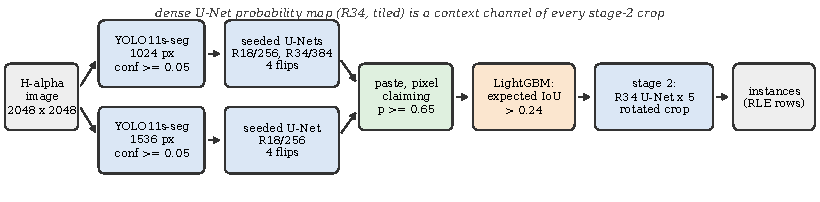
\includegraphics[width=\textwidth]{figures/fig_pipeline.pdf}
  \caption{Data pipeline at inference. Blue: segmentation networks, orange: learned keep or drop decisions, green: rule-based step.}
  \label{fig:pipeline}
\end{figure*}

\textbf{Pre-processing.} The 2048$\times$2048 gray image is used as is. Networks that work on crops receive, next to the gray crop, a contrast-limited adaptive histogram equalisation (CLAHE) of it. No limb-darkening correction or disk masking is applied.

\textbf{Stage 1: proposals.} Two YOLO11s-seg detectors \cite{yolo11}, COCO-pretrained and fine-tuned at 1024~px and 1536~px input, propose boxes with confidence of 0.05 or more. The threshold is low on purpose: recall matters here and the keep decision is taken later. Each annotator view is a separate training sample.

\textbf{Stage 1: crop refinement.} The detector masks are coarse (predicted at a quarter of the input resolution), so every box is segmented again in its own crop by a box-seeded U-Net \cite{unet} with a ResNet encoder \cite{resnet}. Its input is the gray crop, the CLAHE crop and the box mask. For the 1024~px detector a ResNet18 model at 256~px and a ResNet34 model at 384~px are averaged, for the 1536~px detector a ResNet18 model at 256~px is used, each over four flips.

\textbf{Paste.} Candidates of both detectors are pasted into one label image in order of detector score at probability 0.65. A pixel belongs to the first candidate that claims it and instances under 96~px are dropped, so instances never overlap and duplicates of the two detectors collapse.

\textbf{Selection value.} A LightGBM regressor \cite{lightgbm} predicts, for every pasted instance, its matched IoU averaged over the annotator views of the image (zero for a view in which it matches nothing). This is the expected contribution of the instance to the numerator of PQ. The 17 features are detector score, refiner confidence, size, shape, contrast and the agreement of detector mask and refiner mask. Instances with a value at or below $\tau=0.24$ are dropped.

\textbf{Stage 2: re-segmentation in context.} Each kept instance is cut out along its principal axis into a 384$\times$128 crop, so that every filament is horizontal and fills the crop. A U-Net with a ResNet34 encoder receives five channels: gray, CLAHE, the probability map of a dense full-image U-Net (ResNet34, tiled inference), the instance's own stage-1 mask, and the masks of the other kept instances. It is trained with binary cross-entropy plus Dice loss on a soft target: the mean, over the annotator views that contain this filament (IoU above 0.2 with the instance), of the best-overlapping label. The target is thus the share of annotators who marked each pixel. Five fold models and four flips are averaged and thresholded at 0.40.

\textbf{Post-processing.} Stage-2 masks replace the stage-1 masks under the same pixel-claiming rule, and each instance becomes one COCO run-length row. No morphological operation, merging rule or hole filling is applied: none of the variants we tried improved the validation score.

\begin{figure*}[t]
  \centering
  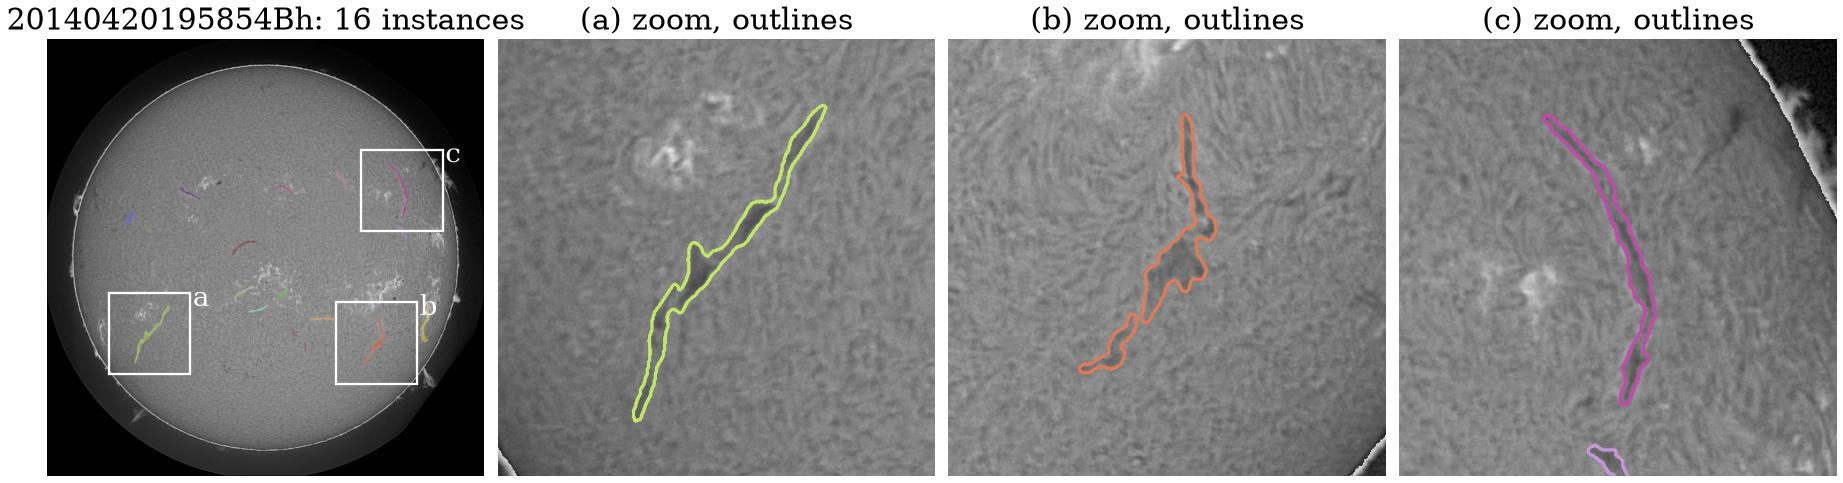
\includegraphics[width=\textwidth]{figures/fig_examples.jpg}
  \caption{Predicted instances for test image 20140420195854Bh (left, one colour per instance) and three zooms with instance outlines.}
  \label{fig:examples}
\end{figure*}

\textbf{Data and sampling.} Only the training split of the competition data was used: 707 images, 1,154 annotator views and 8,199 labelled filaments. No external images or labels, no public MAGFiLO test labels and no hard-coded predictions were used. Pretrained initialisations are public (COCO for YOLO11, ImageNet for the ResNets). There is no fixed validation set. The 707 images are split into five folds, grouped by image so that all views of an image share a fold. For every fold a detector, its refiners and the stage-2 models are trained on the other four folds, which yields out-of-fold predictions for all 707 images. The selector is trained on these out-of-fold candidates with a second grouped five-fold split, so the candidates it learns from have the quality it will meet at test time. Test predictions come from the same recipes trained on all 707 images (detectors, refiners, dense U-Net), from the five fold models averaged (stage 2) and from the selector trained on all out-of-fold candidates. Figure~\ref{fig:examples} shows predictions on a test image.

% ==================================== %
%              EVALUATION              %
% ==================================== %
\section{Evaluation}\label{sec:evaluation}
\textbf{Strategy.} Every number below is out of fold on all 707 training images and is computed like the competition scorer: each annotator view is scored separately and pooled, with matches at IoU above 0.5. Dice and IoU ``per view'' compare the union of predicted instances with the union of one annotator's labels; this Dice equals \texttt{torchmetrics.segmentation.DiceScore} (a test in the repository checks it). Intervals are 95\% percentile intervals of a bootstrap over images (4,000 resamples).

\begin{table}[t]
  \caption{Out-of-fold results on 707 images and 1,154 views, with 95\% bootstrap intervals.}
  \label{tab:main}
  \centering\small
  \begin{tabular}{lcc}
    \toprule
    Metric & Value & 95\% interval \\
    \midrule
    Panoptic Quality & 0.4626 & 0.454 to 0.471 \\
    Segmentation quality (mean IoU of matches) & 0.686 & 0.683 to 0.689 \\
    Recognition quality & 0.674 & 0.662 to 0.686 \\
    Mean Dice per view & 0.655 & 0.643 to 0.666 \\
    Mean IoU per view & 0.505 & 0.494 to 0.516 \\
    \midrule
    Median Dice per view & 0.688 & \\
    Dice pooled over all pixels & 0.686 & \\
    Pixel precision / recall & 0.728 / 0.648 & \\
    TP / FP / FN & \multicolumn{2}{c}{5,295 / 2,210 / 2,904} \\
    Public leaderboard PQ & 0.41 & \\
    \bottomrule
  \end{tabular}
\end{table}

\textbf{Results.} Table~\ref{tab:main} gives the main scores and Figure~\ref{fig:metrics} the distributions. Dice per view has quartiles 0.596 and 0.761; the 28 views below 0.1 are views with few or no labels in which the model predicted filaments, or the reverse. Matched pairs have a mean IoU of 0.686 (mean Dice 0.811). Table~\ref{tab:ablation} shows how the score was built up; every row was measured on the same images. The largest single step is the learned selection.

\begin{figure}[t]
  \centering
  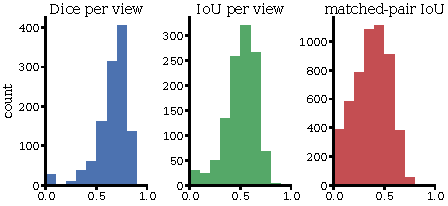
\includegraphics[width=\columnwidth]{figures/fig_metrics.pdf}
  \caption{Distributions over the 1,154 annotator views (Dice, IoU) and over the 5,295 matched pairs (IoU).}
  \label{fig:metrics}
\end{figure}

\begin{table}[t]
  \caption{Out-of-fold PQ of successive versions of the pipeline.}
  \label{tab:ablation}
  \centering\small
  \begin{tabular}{lc}
    \toprule
    Configuration & PQ \\
    \midrule
    One detector and refiner, detector confidence $\geq 0.35$ & 0.4290 \\
    + learned selection value & 0.4547 \\
    + second refiner averaged & 0.4583 \\
    + candidates of the 1536~px detector & 0.4596 \\
    + stage 2 (this submission) & 0.4626 \\
    \bottomrule
  \end{tabular}
\end{table}

\textbf{One-to-many and many-to-one relations.} A prediction lies inside a label when more than half of its pixels do, and the reverse. Of the 8,199 labels, 115 (1.4\%) hold two or more predictions (fragmentation), and 191 of the 7,505 prediction and view pairs (2.5\%) hold two or more labels (merging). Splitting and merging are therefore rare. The dominant errors are labelled filaments without a prediction and predictions that no annotator of that view drew.

\begin{table}[t]
  \caption{Causes of the errors of stage~1 (out of fold, 2,213 false positives and 2,979 false negatives).}
  \label{tab:errors}
  \centering\small
  \begin{tabular}{lr}
    \toprule
    False positives & Share \\
    \midrule
    Fragment of a larger labelled filament & 32\% \\
    No label nearby in this view & 31\% \\
    Matches another annotator's label of the image & 18\% \\
    Covers a label but is much larger & 14\% \\
    IoU just under 0.5 & 5\% \\
    \midrule
    False negatives & Share \\
    \midrule
    Good candidate existed, dropped by the keep rule & 25\% \\
    Only a poor candidate existed & 21\% \\
    Partly covered by a kept prediction & 20\% \\
    Inside a larger kept prediction & 16\% \\
    No candidate & 13\% \\
    IoU just under 0.5, or split & 5\% \\
    \bottomrule
  \end{tabular}
\end{table}

\textbf{Public leaderboard.} The submitted file scores 0.41 on the public half of the test set, against 0.463 out of fold. We see the same gap for every version of the pipeline. Random 90-image subsets of the out-of-fold results have a standard deviation of 0.011 and never fall below 0.415 in 20,000 draws, and year, site and number of annotators are distributed alike in training and test data, so we cannot attribute the gap to sampling. We report it as an open observation.

\textbf{Efficiency.} On one GPU (NVIDIA L40S) the full pipeline takes 1.0~s per 2048$\times$2048 image (5 minutes for the 180 test images, model loading included). Run from the repository weights in a fresh environment, it reproduces the submitted file: 1,214 of 1,214 submitted instances are matched, with a mean IoU of 0.9995 (1,091 masks are identical; the rest differ by a few boundary pixels because of GPU arithmetic). The rerun holds 2 additional instances whose keep value lies at the threshold. On a CPU it takes about 50~s per image.

\textbf{Strengths.} (i) The keep rule optimises the competition metric directly and is trained on the disagreement between annotators instead of ignoring it. (ii) Instances are disjoint by construction, and splitting and merging are rare. (iii) Every component was accepted only after an out-of-fold gain on all 707 images, and the whole pipeline is one class (\texttt{FilamentPipeline}) that reproduces the submitted file from the weights in the repository.

\textbf{Weaknesses and possible improvements.} (i) Recognition, not outline quality, limits the score. Table~\ref{tab:errors} classifies the errors: for a quarter of the false negatives a good candidate existed and was dropped, and 18\% of the false positives match the label of \emph{another} annotator of the same image, so part of the error is annotator disagreement that no model can remove. A perfect keep rule on our candidates would reach about 0.53; closing that gap needs information about annotator behaviour that we could not extract from the image. (ii) Thresholds (selection 0.24, paste 0.65, stage~2 0.40) were chosen on the same out-of-fold predictions that are reported, each from a handful of values, so the reported PQ is slightly optimistic. (iii) The pipeline has several stages and twelve weight files; distilling it into one network would simplify use. (iv) Thin barbs are often cut, because the mean-annotator target rewards the filament body. A target that weights barbs, or labels with annotator identity, would address this. (v) A heavier stage~2 helps: replacing the U-Net by fine-tuned SAM~2.1 models and adding their mask-quality score to the keep rule raises the out-of-fold PQ by 0.010 (95\% interval 0.007 to 0.013, paired bootstrap) at about nine times the run time. That variant is documented in the repository notes; this submission is the faster configuration.

% ==================================== %
%            ACKNOWLEDGMENT            %
% ==================================== %
\section{Acknowledgment}\label{sec:acknowledgment}
% Do not change
The organization of the Filament Segmentation Challenge 2026 is partially supported by the U.S. National Science Foundation (NSF) under Grant No. 2209912 and 2433781, directorate for Computer and Information Science and Engineering (CSE), and Office of Advanced Cyberinfrastructure (OAC), and Grant No. 2511630, AST Division Of Astronomical Sciences and MPS Directorate for Mathematical and Physical Sciences.

The Filament Segmentation Challenge 2026 is sponsored by the U.S. National Science Foundation (NSF) National Solar Observatory (NSO).

This work utilizes GONG data obtained by the NSO Integrated Synoptic Program, managed by the National Solar Observatory, which is operated by the Association of Universities for Research in Astronomy (AURA), Inc. under a cooperative agreement with the National Science Foundation and with contribution from the National Oceanic and Atmospheric Administration. The GONG network of instruments is hosted by the Big Bear Solar Observatory, High Altitude Observatory, Learmonth Solar Observatory, Udaipur Solar Observatory, Instituto de Astrof\'isica de Canarias, and Cerro Tololo Interamerican Observatory.

\bibliographystyle{ACM-Reference-Format}
\bibliography{main,refs}

\end{document}
